% !TEX program = xelatex
\documentclass{article}
\usepackage[utf8]{inputenc}
\usepackage{amsmath}
\usepackage{relsize}
\usepackage{amssymb}
\usepackage{mathabx}
\usepackage{amsthm}
\usepackage{graphicx}
\usepackage[usenames,dvipsnames]{xcolor}
\usepackage{subcaption}
\newcommand{\kacper}[1]{ \bf  { \color{Orchid}{Kc: #1}}  }

\newtheorem{definition}{Definition}
\newtheorem{lemma}{Lemma}
\newtheorem{Theorem}{Theorem}
\newtheorem{example}{Example}
\newtheorem{statement}{Statement}
\newtheorem{corollary}{Corollary}
\newtheorem{test}{Test}
\newtheorem{proposition}{Proposition}

\newtheorem*{remark}{Remark}
\newenvironment{claim}[1]{\par\noindent\underline{Claim:}\space#1}{}
\newenvironment{claimproof}[1]{\par\noindent\underline{Proof:}\space#1}{\hfill $\blacksquare$}

\title{Testing MCMC convergence}
\author{}
\date{}

% TODO 
% Wrong disitbution under null if ratio is not good


\begin{document}

\maketitle




Let $g(x,y)$ be a characteristic, analytic kernel. Let $p$ be a probability measure on $R^d$; suppose it has a density which logarithm exists, and is differentiable. Consider the following transform of $R^d$ valued random variable $X$
\begin{align}
 \mu_p(y) = E  \nabla \log p(X) g(X,y) - E \nabla g(X,y)
\end{align}
this transform is closely connected to Stein method and kernel mean embedding. Actually, as Arthur has showed in his note this is a mean embedding. But latter I think the distance squared should be different
\begin{align}
&d_q(p) = \\
&= E \langle   \frac{\partial } {\partial x_1} \log p(X_1) k(X_1,\cdot) + \frac{\partial } {\partial x_1} k(X_1,\cdot) ,  \frac{\partial }{\partial x_2} \log p(X_2) k(\cdot,X_2) +  \frac{\partial } {\partial x_2} k(\cdot,X_2) \rangle \\
  &= E  \frac{\partial } {\partial x_1} \log p(X_1) \frac{\partial } {\partial x_2} \log p(X_2) k(X_1,X_2) +
          \frac{\partial } {\partial x_2} p(X_2) \frac{\partial } {\partial x_1} k(X_1,X_2) \\
  &+  \frac{\partial } {\partial x_1} \log p(X_1) \frac{\partial } {\partial x_2} k(X_1,X_2) + \frac{\partial } {\partial x_1}\frac{\partial } {\partial x_2} k(X_1,X_2)
\end{align}
this make more sense when we write it this way
\begin{align}
 E \frac{\partial } {\partial x_1} \log p(X_1) g_1(X_1,X_2) + \frac{\partial } {\partial x_1} g_1(X_1,X_2) + \\
 E \frac{\partial } {\partial x_1} p(X_1) g_2(X_1,X_2) +  \frac{\partial } {\partial x_1}\frac{\partial } {\partial x_2} g_2(X_1,X_2)
\end{align}
where 
$$
g_1(x_1,x_2) = \frac{\partial } {\partial x_2} \log p(x_2) k(x_1,x_2)
$$
and
$$
g_2(x,x') = \frac{\partial } {\partial x_2} k(x_1,x_2)
$$
Now,once we condition of $X_2$,  its easy to see that the core of U-statistic is degenerate, since $g_1(x,\cdot)$ and $g_2(x,\cdot)$ are just arbitrary functions as in Stein method.  
$$
E \left (\frac{\partial } {\partial x_1} \log p(X_1) g_1(X_1,X_2) + \frac{\partial } {\partial x_1} g_1(X_1,X_2) \right )| X_2 = 0
$$
$$
E \left ( \frac{\partial } {\partial x_1} p(X_1) g_2(X_1,X_2) 
+  \frac{\partial } {\partial x_1}\frac{\partial } {\partial x_2} g_2(X_1,X_2) \right )| X_2 = 0
$$
To understand the behaviour under alternative it is sufficient to notice that mean embedding is surely not zero. Suppose $X \sim q$
\begin{align}
 &E \frac{\partial } {\partial x_1} \log p(X_1) k(X_1,t) + \frac{\partial } {\partial x_1} k(X_1,t) =\\
 &E  \frac{\partial } {\partial x_1} ( \log  p(X_1) + \log  q(X_1)- \log  q(X_1)  )  k(X_1,t)   + \frac{\partial } {\partial x_1} k(X_1,t) = \\
 &E  \frac{\partial } {\partial x_1} (\log p(X_1) - \log q(X_1))k(X_1,t)   = \\
 & \int  (\log p(x) - \log q(x) ) k(x,t) p(x) dx
\end{align}
The integral transform is zero is and only $\log p(x) = \log q(x)$ for a right class of kernel.

\section{test}
For some fixed location $y$ and a random variable $X$, define a random variable $s(X,y)$
\begin{align}
 s(X,y) = \nabla \log p(X) g(X,y) -  \nabla g(X,y).
\end{align}
For some number of random locations $Y_1,Y_J$ and a random variable $X$ define a random vector $Z_i$
\begin{equation}
 Z_i = ( s(X_i,Y_1) , \cdots, s(X_i,Y_J)  )\in \mathbf R^J.
\end{equation}

Let $W_n$ be a mean of $Z_i$'s
$W_n = \frac 1  n \sum_{i=1}^n Z_i, $
and $\Sigma_n$ its  covariance matrix
$\Sigma_n = \frac 1  n Z Z^{T}$.
The test statistic is
\begin{equation}
 S_n = n W_n \Sigma_n^{-1} W_n.
\end{equation}
The computation of $S_n$ requires inversion of a $J\times J$ matrix $\Sigma_n$, but this is fast and numerically stable: $J$ will typically be small, and is less than 10 in our experiments. The next proposition demonstrates the use of $S_n$ as a one-sample test.
\begin{proposition}[Asymptotic behavior of $S_n$]
\label{prop:Hotelling}
 If  $E s(X,y)=0$ for all $y$, then the statistic $S_n$ is a.s. asymptotically distributed as a $\chi^2$-random variable with $Jd$ degrees of freedom, where $d$ is $X$ dimensionality (as $n \to \infty$ with $d$ fixed). If  $E s(X,y) \neq 0$ for almost all $y$ then a.s. for any fixed $r$, $\mathbb P(S_n > r) \to 1$  as $n \to \infty$ .
\end{proposition}


\begin{test}[One sample test]
\label{test}
Calculate $S_n$. Choose a threshold $r_\alpha$ corresponding to the $1-\alpha$ quantile of a  $\chi^2$ distribution with $J$ degrees of freedom, and reject the null hypothesis whenever $S_n$ is larger than $r_\alpha$. 
\end{test}

\section{Experiments}

\subsection{Student's t vs Normal}
In this  sanity check we replicate the experiment 4.1 from \cite{gorham2015measuring}. The null hypothesis is that observed samples $x_i$, for $1 \leq i \leq 500$ come from standard normal distribution. We will check the power of the one-sample test by generating samples from Student's t distributions with increasing number of degrees of freedom, and analyzing p-values. For the Student's t distribution with a number of degrees of freedom $\nu$, we draw 500 samples and calculate the p-value -- this procedure is repeated 150 times so 150 p-values are calculated and a bar plot of p-values is created. The number of degrees of freedom $\nu$ varies in the range $1,6,\cdots,71$ and bar plots for each of $\nu$ is drawn.  The results are plotted in the figure \ref{fig:studentst}. The bar plot for $\nu = inf$ is calculated for samples coming from normal distribution.

\begin{figure}
\label{fig:studentst}
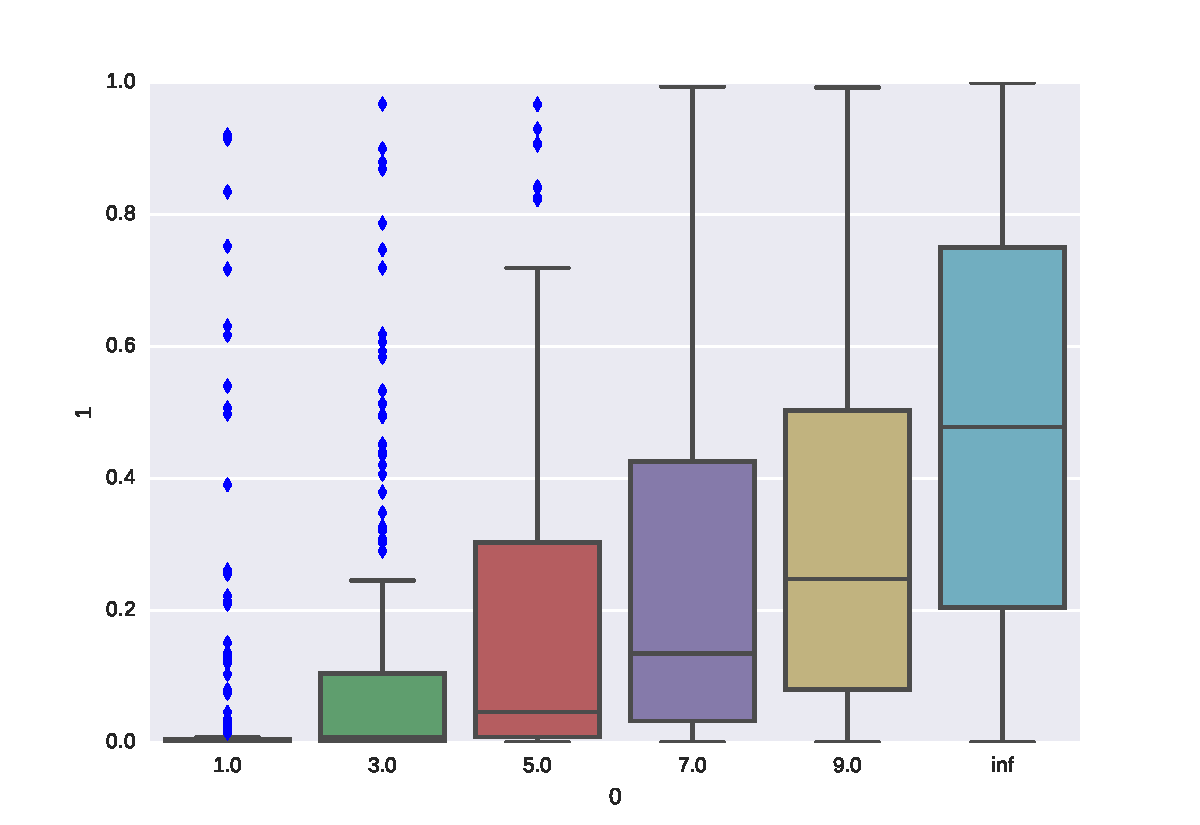
\includegraphics[width=0.8\textwidth]{./img/student.pdf}
\caption{Distribution of p-values as a function of number of degrees of freedom.}
\end{figure}

\subsection{MCMC diagnostic}
This one sample test can be used for diagnostics of most of the MCMC methods. In the following experiment we will demonstrate how to verify if the samples obtained form two sampling can be assumed to come from the stationary distribution.  

Here we model used in the experiment 5.1. The model is 
\begin{align}
 \theta_1 \sim N(0,10) ; \theta_2 \sim N(0,1)
 X_i \sim \frac {1}{2} N(\theta_1,4) + \frac{1}{2} N(\theta_2,4) 
\end{align}
400 points are drawn from this model. In the following experiment we would like to characterize the average time required for convergence for two different MCMC algorithms. In order to do so we run multiple chains and asses distribution of p-values. Under the null hypothesis p-values should have uniform distribution and, as in the previous experiment, we asses the divergence of the p-values from the uniform by bar plots. Formally for both methods plain MH and SGLD we generate $40 \times 100$ chains. We divide those chains into $40$ groups of $100$ chains and run one-sample tests for for predefined times $t_1,...,t_10$  so that for each of group we get p-values at ten different times. Then we plot those p-values jointly on plots a and b. We don't use thinning.  


\paragraph{Metropolis Hastings with random walk}
We use plain MH MCMC with Gaussian proposal with with standard deviation equal to  $0.2$.   

\subsection{SGLD, plain }
Stochastic gradient  Stochastic Gradient Langevin Dynamics  with schrinking step size $\epsilon_t$ is a MCMC procedure desigend for large datasets. 
400 points are drawn from the this model with $\theta_1 = 0$ and $\theta_2= 1$. In such a setting there are two modes in the posteriori disitbiution, one at the the point $0,1$ and the other at the point $1,-1$. We run the SGLD alogrithm with a batch size of 1 and 10000 iterations through the whole dataset. The stepsizes are $\epsilon_t = a(b+t)^{.55}$ where $ a = 0.01584$ and $b=2.31$ such that $\epsilon_t$ deacreses from $0.01$ to $.
0001$. 


\begin{figure}
\begin{subfigure}{.5\textwidth}
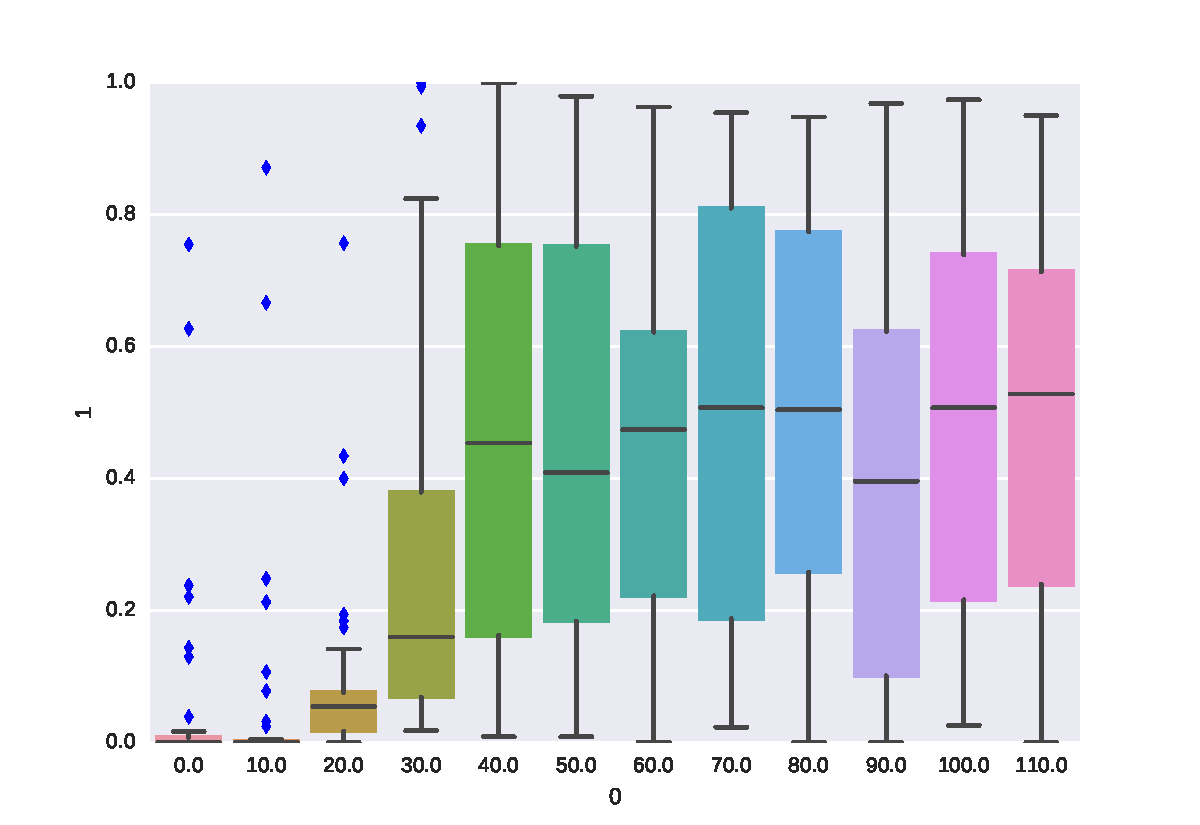
\includegraphics[width=\textwidth]{./img/mcmc_mixing.pdf}
\end{subfigure}%
\begin{subfigure}{.5\textwidth}
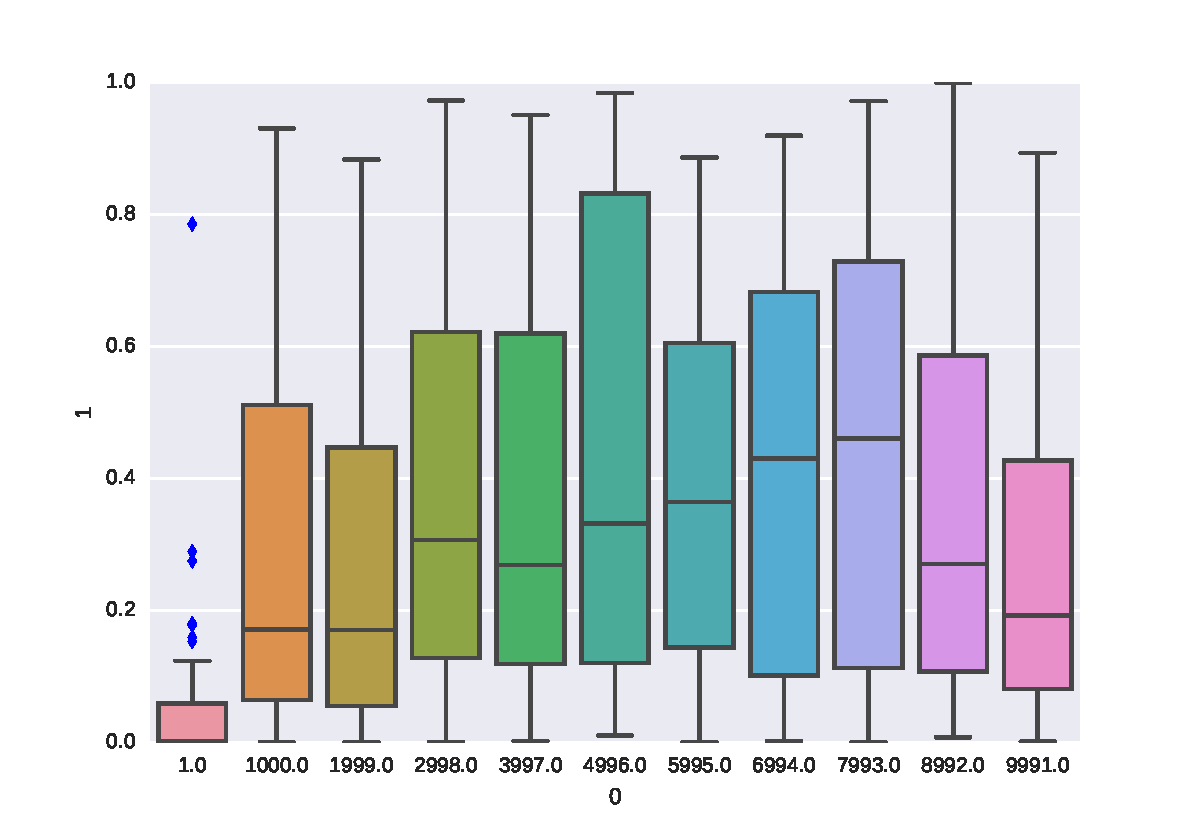
\includegraphics[width=\textwidth]{./img/sgld_mixing.pdf}
\end{subfigure}%
\end{figure}


\begin{figure}
\begin{subfigure}{.5\textwidth}
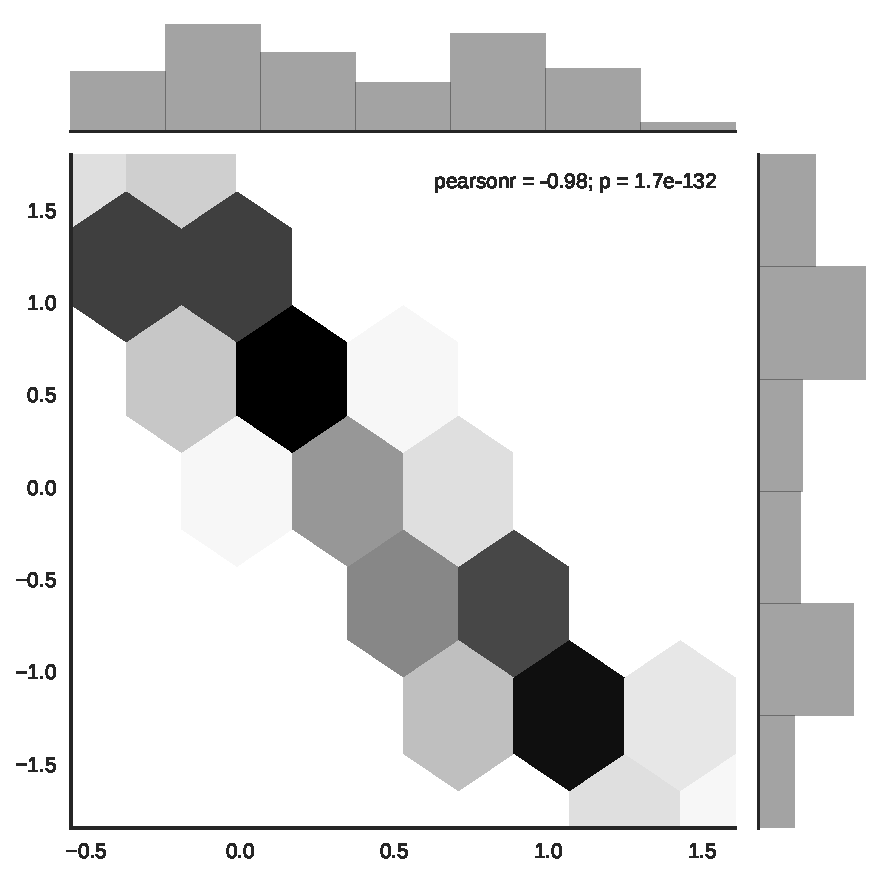
\includegraphics[width=\textwidth]{./img/mcmc_sample.pdf}
\end{subfigure}%
\begin{subfigure}{.5\textwidth}
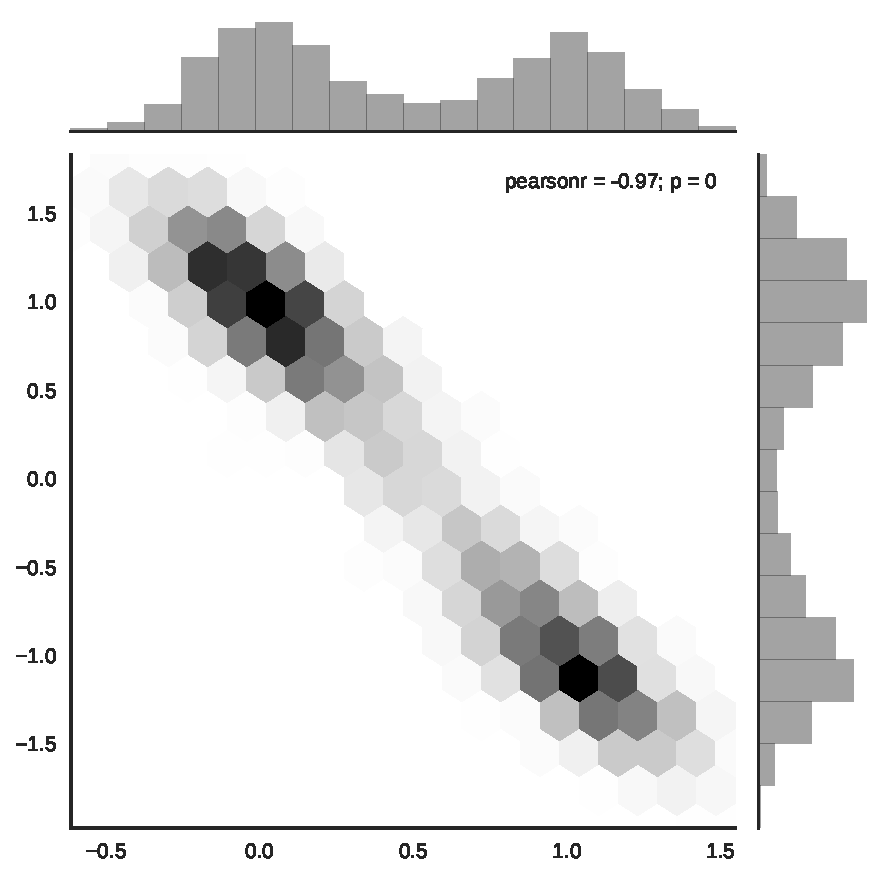
\includegraphics[width=\textwidth]{./img/sgld_sample.pdf}
\end{subfigure}%
\end{figure}




\section{Math}

\begin{statement}
 If $X$ is distributed according to $p$ then the function  $\mu_p(y)$ is identically equal to zero  
\end{statement}
\begin{proof}
 For a fixed $y$ this is consequence of Stein method with as described in those guys NIPS paper. Or one can do integration by parts.   
\end{proof}

\begin{statement}
 If $X$ is not distributed according to $p$, but has a density, then $\mu_p(y)$ is different form zero almost everywhere. 
\end{statement}
\begin{proof}
THIS IS A SKETCH-- which means it's technically not a proof, but you may convince yourself it's true (if it is, but code seems to approve).
 Suppose $X$ is distributed according to density $p'$, then

\begin{align}
\mu_p(y) =& \int_{R^d} ( \nabla \log p(x) g(x,y) -  \nabla g(x,y)) p'(x) dx \\
          & \int_{R^d} g(x,y) \frac{ p'(x)}{p(x)} \nabla p(x) - \nabla g(x,y) p'(x)  
\end{align}
Integration by parts and shows that for all partial derivatives 
\begin{align}
0 = \int_{R} \frac{ \partial g(x,y)p'(x)} { \partial x_i } dx_i
\end{align}
\begin{align} 
 \int_{R} \frac{ \partial g(x,y) } { \partial x_i } p'(x) d x_i =
 -\int_{R} \frac{ \partial p(x) } { \partial x_i } g(x,y) d x_i 
\end{align}
So
\begin{align}
\mu_p(y) =& \int_{R^d} g(x,y) \frac{ p'(x)}{p(x)} \nabla p(x) -  g(x,y) \nabla p'(x)  \\
	 =& \int_{R^d} g(x,y) \left( \frac{ p'(x)}{p(x) } \nabla p(x) -  \nabla p'(x) \right)
\end{align}
 We would like to say that $t(x) = \frac{ p'(x)}{p(x) } \nabla p(x) -  \nabla p'(x)$  is kind of bounded and invoke the argument that $\mu_p$ is analytic, but first we need to prove that $t(x)$ is non-zero. 
 It is sufficient to see that $t(x) =0$ implies that $\nabla [ \log( p(x)) - \log( p'(x)) ]=0$, which implies that $p(x) = p'(x)e^C$. Since both $p$ and $p'$ are probability measures,  $C$ must be equal to 0.
 
 $\mu_p$ lives in the $RKHS$ associated with kernel $g$. Indeed if the integral exists 
 \[
  \int f(x) t(x) 
 \]
 then there exist an element $\mu_t$, such that $<\mu_t, f>$ is equal to above integral and in addition to that 
 \[
  \mu_t(t) = < \mu_t, k(t,\cdot)> = \int k(t,x) t(x) = \mu_p(t). 
 \]
The sufficient condition for $\int f(x) t(x)$ to exist is that 
\[
 \int <f, k(x,)> t(x) = < f, \int k(x,) t(x) > 
\]
$\int k(x,) t(x) $ exists and this one is easily verifiable for popular kernel (e.g. exists for exponential families and Gaussian kernel). By the lemma form our previous paper we see that $\mu_p(t)$ is  analytic. 
\end{proof}

\paragraph{Temporal dependence -- not an issue}
There are several ways to deal with temporal dependence, all of which, to our knowledge, work only asymptotically. Options include estimating auto-covariances, performing bootstrap or thinning. The last one, usually avoided in time-series analysis due to it's wasteful approach to data, is quite feasible in this application. It is also equally or less computationally complex then other options (potentially less noisy then estimating the auto covariance).      

It's obvious, but needs to show formally, that distribution of the test statistic under the null hypothesis, as $n$ approaches infinity, is as if we had used IID data. This is proved in appendix.

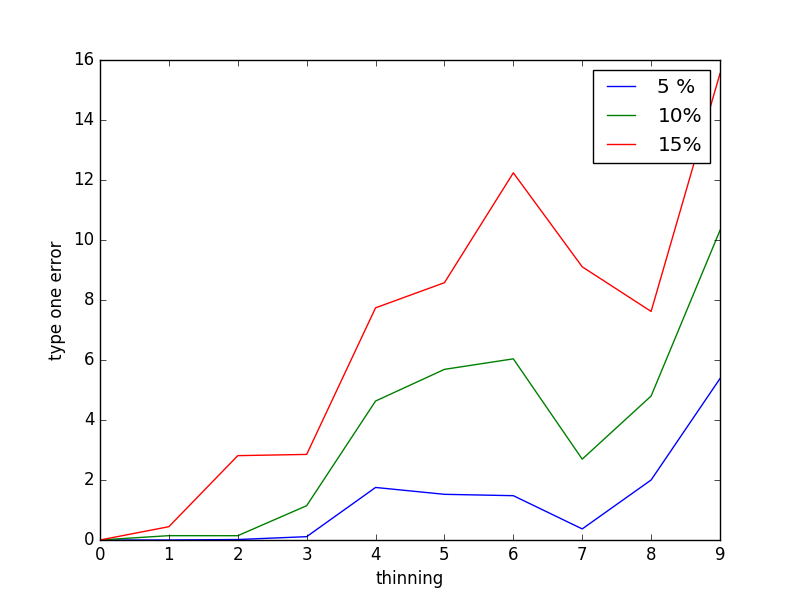
\includegraphics[width=0.8\textwidth]{type1.png}

\section{Sample selection}
So far we have not discussed problem problem of selecting sample from stationary distribution. In this section we propose a procedure that returns a sample for which it can not be rejected that it was generated from null distribution. We will proceed similarly to Heidelberger-Welch procedure, but is simpler way. We will generate blocks of samples and run test on them until we accept of world ends. 

\paragraph{type One-error}
We will use simple Bonferroni correction to deal with type one error. Tests level must be adjusted, so that they sum up to $\alpha$. Any scheme can be used, we use $\frac{1}{x^2}$ since we believe (am I turning  Bayesian?) that chains converge fast on average (faster than precision of the test that we are using).   

\paragraph{Type two}
Type two is somehow more complicated. In general (this is my intuition from finite state Markov chains and AR processes ) chain does not converge to stationary distribution in any number of finite steps, unless it has started for the stationary distribution. As usually in testing, one has no finite sample control over type two error. We can however infer what misspecified log probability would have given similar results on the given sample. This can be done by perturbing log probability in some direction and calculating the statistic on our sample. The magnitude of perturbation will show which models appear to be indistinguishable (now talk about parameters inference and that its even more difficult )    







\bibliographystyle{plain}
\bibliography{biblio}










\end{document}


